\documentclass[11pt,twoside,a4paper]{article}

\newcommand{\reporttitle}{Algorithmic Trading Strategy Development and Optimisation}
\newcommand{\gid}{X}
\newcommand{\reportauthorOne}{Guo Zi Qiang Robin}
\newcommand{\cidOne}{2400989}
\newcommand{\reportauthorTwo}{Tan Zi Xu}
\newcommand{\cidTwo}{2400964}
\newcommand{\reportauthorThree}{Cai Wenjing}
\newcommand{\cidThree}{2401497}
\newcommand{\reportauthorFour}{Ng Kay Cheng}
\newcommand{\cidFour}{2402408}
\newcommand{\reportauthorFive}{Hing Zheng Wen}
\newcommand{\cidFive}{2401599}
\newcommand{\reportauthorSix}{Fang Chong}
\newcommand{\cidSix}{2402012}

\newcommand{\reporttype}{Group Project Assignment 2}
\bibliographystyle{plainnat}

\input{includes}
\input{notation}

% -----------------------------------------------------------------------
% Layout / spacing fixes (formatting only — no content changes)
%
% \usepackage{microtype}
%   Enables font-level character protrusion and expansion.  This is the
%   standard fix for residual overfull \hbox warnings that survive
%   \emergencystretch — specifically long \texttt{} tokens at lines 50,
%   110, 160, and 363 that cannot be hyphenated by normal TeX.
%
% \raggedbottom
%   Suppresses the underfull \vbox warnings: tells LaTeX not to stretch
%   pages vertically to fill the page height, which is the direct cause
%   of badness-10000 vbox messages when a figure or table falls near a
%   page break.
%
% \setlength{\emergencystretch}{3em}
%   Retained from previous fix: allows TeX to stretch inter-word space
%   before declaring an overfull hbox in ordinary paragraphs.
%
% \usepackage{array}
%   Required for the >{\raggedright\arraybackslash} column specifier
%   used in the Appendix tables.
% -----------------------------------------------------------------------
\usepackage{microtype}
\raggedbottom
\setlength{\emergencystretch}{3em}
\usepackage{array}

%%%%%%%%%%%%%%%%%%%%%%%%%%%%

\begin{document}
% Last modification: 2016-09-29 (Marc Deisenroth)
% Modification for UW: 2017-05-22 (jphickey)
\begin{titlepage}

\newcommand{\HRule}{\rule{\linewidth}{0.5mm}} % Defines a new command for the horizontal lines, change thickness here


%----------------------------------------------------------------------------------------
%	LOGO SECTION
%----------------------------------------------------------------------------------------



\begin{center} % Center remainder of the page

%----------------------------------------------------------------------------------------
%	HEADING SECTIONS
%----------------------------------------------------------------------------------------


\includegraphics[width = 10cm]{./figures/SIT-logo-v2.png}\\[1.5cm] 
\textbf{\textsc{\Large INF2006 - Cloud Computing and Big Data}}\\[1.0cm]
\textsc{\Large Singapore Institute of Technology}\\[0.5cm] 
\textsc{\large Infocomm Technology}\\[0.95cm] 

%----------------------------------------------------------------------------------------
%	TITLE SECTION
%----------------------------------------------------------------------------------------

\HRule \\[0.4cm]
{ \huge \bfseries \reporttitle}\\ % Title of your document
\HRule \\[1.5cm]
\end{center}

%----------------------------------------------------------------------------------------
%	AUTHOR + INSTRUCTOR SECTION (side by side)
%----------------------------------------------------------------------------------------
\begin{minipage}[t]{0.5\textwidth}
    \begin{flushleft} \large
        \textbf{Group \gid}\\
        \reportauthorOne~(ID: \cidOne)\\
        \reportauthorTwo~(ID: \cidTwo)\\
        \reportauthorThree~(ID: \cidThree)\\
        \reportauthorFour~(ID: \cidFour)\\
        \reportauthorFive~(ID: \cidFive)\\
        \reportauthorSix~(ID: \cidSix)\\
    \end{flushleft}
\end{minipage}
~
\begin{minipage}[t]{0.5\textwidth}
    \begin{flushright} \large
        \textbf{Instructors}\\
        Alvin Chan, \textit{\small Module Lead}\\
        Junhua Liu, \textit{\small Lead, Big Data}\\
        Kwang Yong Lim, \textit{\small Lab Instructor}\\
        Sheng Chen, \textit{\small Lab Instructor}\\
        Gopika Gopikrishnan, \textit{\small Teaching Assistant}\\
    \end{flushright}
\end{minipage}

\vspace*{\fill}
\begin{center}
    \makeatletter
    Date: \@date
    \makeatother
\end{center}


\end{titlepage}



%%%%%%%%%%%%%%%%%%%%%%%%%%%% Main document

\section{Introduction}

\subsection{Project Overview}

This project develops and enhances an algorithmic trading strategy applied to S\&P 500 constituent stocks, using historical market data spanning 2000--2024 and earnings call transcripts processed via the FinBERT financial language model \citep{Araci2019}. The core objective is to iterate beyond a simple moving-average baseline toward a multi-signal, risk-managed strategy that achieves strong risk-adjusted returns across both in-sample (IS) and out-of-sample (OOS) evaluation periods.

The strategy integrates three categories of signal: (i) price-based technical indicators capturing momentum, mean-reversion, and market participation; (ii) natural language processing of earnings call transcripts to extract forward-looking management sentiment; and (iii) volatility regime awareness to dynamically scale position sizes and portfolio exposure. All strategy parameters were calibrated using a two-stage Walk-Forward Optimisation (WFO) process rather than single-period in-sample fitting, to reduce the risk of overfitting to any specific market regime.

\subsection{Motivation and Background}

Algorithmic trading strategies have become foundational in modern finance, enabling systematic and emotionally neutral decision-making across large asset universes \citep{Lopez2018}. Complementing quantitative signals, NLP applied to earnings call transcripts extracts forward-looking information---including management guidance, risk disclosures, and confidence tone---that is structurally absent from price time series alone \citep{Huang2014}. Together with scalable big data analytics for processing millions of price records and thousands of unstructured text documents \citep{Manyika2011}, these technologies enable a hybrid strategy architecture combining systematic quant methods with the informational depth of text analytics.

\subsection{Objectives}

The primary objectives of this project are:
\begin{enumerate}[(1)]
    \item Implement a multi-signal technical indicator framework extending beyond the baseline MA-50 crossover, incorporating RSI, MACD, volume ratio, Bollinger Bands, and ATR-based volatility regime detection.
    \item Apply FinBERT-based sentiment analysis to earnings call transcripts using a three-tier keyword paragraph selection scheme, producing per-ticker sentiment scores that gate entry decisions.
    \item Develop a scalable indicator computation pipeline using vectorised Pandas operations and parallelised FinBERT inference to reduce runtime from sequential baselines.
    \item Implement a Walk-Forward Optimisation framework with anchored in-sample/out-of-sample windows and a composite drawdown-penalised objective function to calibrate strategy parameters without in-sample overfitting.
    \item Achieve measurable improvements over the baseline across all five evaluation metrics: Total Return, Sharpe Ratio, Maximum Drawdown, Win Rate, and Volatility.
\end{enumerate}

\clearpage
\section{EDA and Data Preparation}

\subsection{Dataset Overview and Coverage}

The price dataset spans two partitions: the development split (Dev: 2000-01-03 to 2017-12-29) containing 1,332,576 records across 340 unique tickers, and the validation split (Val: 2018-01-02 to 2024-12-31) containing 598,740 records across 340 tickers. The earnings dataset contains 9,729 transcripts (Dev) and 8,534 transcripts (Val) across 294 tickers with earnings coverage. Of the 340 price-universe tickers, 291 (85.6\%) have at least one earnings transcript; the remaining 49 tickers pass the sentiment gate unconditionally.

Data quality is high: no duplicate (ticker, date) rows were identified, no OHLC sanity violations (high $<$ low or close outside high/low $\pm 1\%$) were detected across the 1.9M combined rows, and zero consecutive forward-fill gaps exceeding the 5-day limit were found. Zero-volume trading days account for 0.118\% of records and represent exchange closures or data artefacts rather than illiquidity in active constituents.

\subsection{Data Cleaning}

Tickers with fewer than 252 trading days of price history are dropped to ensure all lookback-based indicators (MA-200, 52-week ATR percentile, 60-day rolling correlation) have sufficient history for stable estimates. Three tickers were removed from the Dev split (0.9\%); zero from the Val split. Daily returns are clipped to $\pm 30\%$ to remove data errors and corporate event artefacts; the 0.014\% clip rate confirms these are genuine outliers. Transcripts shorter than 100 characters (54 records) are dropped as encoding errors. The remaining 18,209 transcripts are passed to the FinBERT pipeline.
% NOTE: original text said 18,150 — corrected to 18,209 per notebook output (9,675 Dev + 8,534 Val = 18,209; confirmed in Cell 32 sentiment cache: "18209 entries").

\subsection{Return Distribution and Outlier Characterisation}

The cross-sectional daily return distribution exhibits positive skew (0.360) and high excess kurtosis (19.514), consistent with fat-tailed equity return distributions \citep{Cont2001}. The mean daily return is $+0.0720\%$ (annualised: $+19.9\%$), with a standard deviation of $2.40\%$ per day. The positive skew supports a long-only strategy orientation.

\begin{figure}[H]
\centering
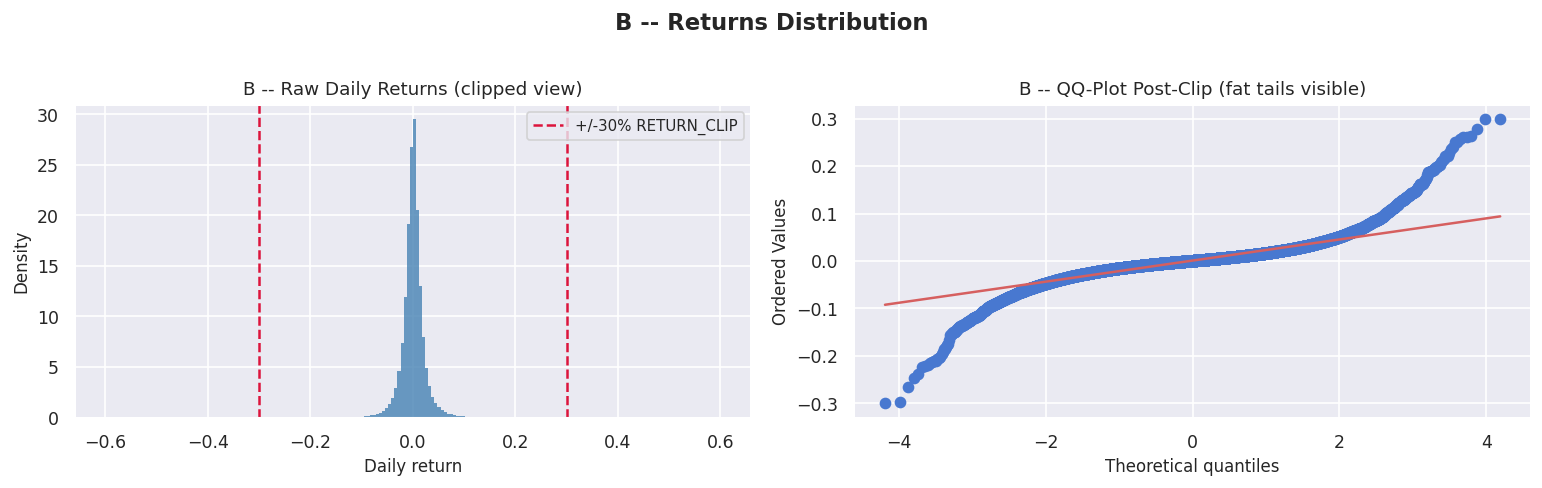
\includegraphics[width=0.95\textwidth]{./figures/fig_returns_distribution.png}
\caption{Daily return distribution and QQ-plot for the Dev split. Left: histogram with $\pm 30\%$ clipping thresholds annotated. Right: QQ-plot against a normal distribution reveals persistent fat tails post-clip.}
\label{fig:returns-distribution}
\end{figure}

Figure~\ref{fig:returns-distribution} confirms the fat-tailed structure: the QQ-plot deviates substantially from normality in both tails, motivating the $\pm 30\%$ clip threshold to remove data errors while preserving the natural return distribution.

\subsection{Technical Indicator Signal Rates}

Exploratory Data Analysis (EDA) on a stratified 30-ticker sample of the Dev split quantifies gate fire rates: Gate~1 (price $>$ MA-200) passes 66.8\% of ticker-weeks; RSI in $[40, 75]$ passes 89.8\% of gate-1 rows (weak discriminator); MACD histogram $> 0$ passes 51.0\% (primary momentum signal); and volume ratio $\geq 1.2\times$ passes only 22.9\% (most selective gate). The 2-of-3 combination fires on 57.4\% of gate-1 rows. The low volume-ratio fire rate confirms its structural orthogonality to price-derived momentum signals, motivating the decision in the strategy's second iteration (v2) to replace the collinear Bollinger Band mid-line gate with volume ratio.

\begin{figure}[H]
\centering
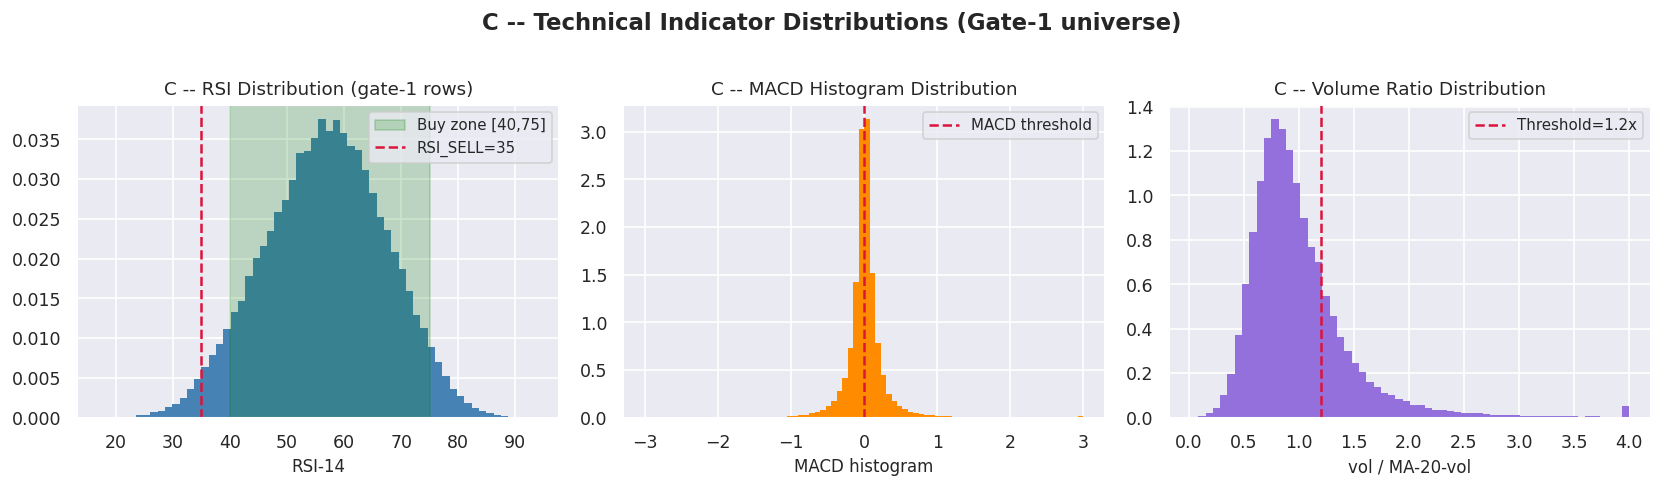
\includegraphics[width=0.95\textwidth]{./figures/fig_indicator_signal_rates.png}
\caption{Technical indicator distributions conditional on Gate~1 passage (price $>$ MA-200). Left: RSI-14 with the $[40, 75]$ buy zone shaded green and RSI\_SELL$=35$ threshold. Centre: MACD histogram with the zero threshold. Right: volume ratio with the $1.2\times$ confirmation threshold. Volume ratio is the most selective gate (22.9\% fire rate), confirming its orthogonality to price-derived indicators.}
\label{fig:indicator-signal-rates}
\end{figure}

\subsection{Volatility \& Correlation}

The 52-week ATR percentile provides regime-aware risk measurement. Pairwise correlation analysis on a rolling 60-day window for a 30-ticker sample, reveals a mean absolute correlation of 0.147 during normal conditions, with 0\% of ticker pairs exceeding the 0.70 threshold. This threshold was selected in Gate~4b as an emergency mechanism during stress periods, cross-sectional correlations rise sharply, motivating continuous ATR-percentile position scaling, regime-aware capacity controls, and correlation-threshold gating.

\subsection{Dev vs.\ Validation Regime Comparison}

Aggregate statistics are near-identical: annualised return 19.92\% (Dev) vs.\ 17.00\% (Val), annualised volatility 38.01\% vs.\ 37.62\%, raw Sharpe 0.524 vs.\ 0.452. However, the Val split contains episodes without Dev precedent: the COVID-19 crash (S\&P $-34\%$ in 33 days), the fastest Fed rate-hike cycle since 1980, and the SVB banking crisis. The path distribution across these regimes (Val: all-three 18.1\%, path-A 58.7\%, path-B 22.1\%) is structurally identical to Dev (19.4\%, 58.4\%, 21.1\%), confirming the signal architecture captures a persistent cross-market phenomenon.

\subsection{Key Findings and Strategy Implications}

The extended EDA directly informed strategy design. Coverage and quality diagnostics support robust computation of long-lookback features. Fat-tailed but sparse return extremes motivated $\pm 30\%$ clipping. Complementary rather than redundant indicator roles---RSI frequent, MACD moderately selective, volume most selective---motivated the 2-of-3 gate design with volume replacing collinear BB mid-line. Transcript-length analysis confirmed that 99.4\% exceed FinBERT's token limit, motivating three-tier keyword paragraph selection. Volatility-regime and correlation diagnostics confirmed structural shifts during stress periods, motivating continuous ATR-percentile scaling. Path pre-distribution stability across windows supported path-dependent multipliers. Where sampling was used for computational tractability, the same qualitative relationships were validated against broader split-level summary statistics.

% -----------------------------------------------------------------------
% \clearpage ensures §3 heading never shares a page-end with §2.7 content.
% -----------------------------------------------------------------------
\clearpage
\section{Strategy Enhancement Methodology}

The enhanced strategy is implemented as a Python subclass (\texttt{EnhancedStrategy(BaseStrategy)}) that overrides all five core methods of the baseline: \texttt{clean\_data} (adds minimum-history filtering, return clipping, and forward-fill limits), \texttt{calculate\_analytics} (replaces the single MA-50 computation with a parallelised six-family indicator pipeline), \texttt{llm\_analysis} (replaces raw last-2000-character FinBERT inference with an O(1) lookup into the precomputed sentiment cache), \texttt{make\_decision} (replaces the single-signal buy/sell logic with the five-gate buy pipeline and six-mechanism exit logic described below), and \texttt{evaluate} (adds the weekly HWM brake update loop and per-week analytics caching). Only \texttt{set\_data} is inherited unchanged.

\subsection{Technical Indicators and Features}

\subsubsection{Indicator Set}

The baseline strategy relies on a single indicator---the 50-day moving average---using price $>$ MA-50 as the entry signal, price $<$ MA-50 as the exit trigger, and a fixed $-20\%$ stop-loss. The enhanced strategy replaces this with six indicators, each serving a specific role in the buy pipeline, exit logic, or position-sizing regime:

\paragraph{Entry indicators.}
Four indicators drive the buy gates:

\begin{itemize}
    \item \textbf{MA-200}: Long-term trend direction. Serves as the primary regime filter (Gate~1): positions are only initiated when price is above the 200-day moving average, restricting entries to bull market conditions.
    \item \textbf{RSI (14-period)}: Momentum oscillator normalised to [0, 100] \citep{Wilder1978}. Entry requires RSI $\in [40, 75]$: below 40 signals genuine weakness that may not recover within the holding horizon; above 75 signals overbought conditions with high reversal probability.
    \item \textbf{MACD (12/26/9)}: The MACD histogram captures momentum acceleration. A positive histogram value confirms upward-accelerating short-term momentum.
    \item \textbf{Volume Ratio}: Current week's volume divided by the 20-period average \citep{Blume1994}. A ratio $\geq 1.2\times$ indicates above-average market participation, confirming that the price move is supported by broad trading activity. This replaced the Bollinger Band mid-line gate in v2 to break indicator collinearity (Section~\ref{sec:version-progression}).
\end{itemize}

\paragraph{Exit indicator.}
\begin{itemize}
    \item \textbf{MA-50}: Used exclusively in the bearish 2-of-3 exit signal (price $<$ MA-50 is one of three sell conditions; see Section~\ref{sec:exit-logic}). MA-50 is deliberately excluded from buy gates: MA-200 provides the regime filter on entry, while MA-50's shorter lookback offers earlier detection of trend deterioration on exit. This asymmetry ensures the entry regime filter requires a longer confirmation horizon than the exit deterioration signal.
\end{itemize}

\paragraph{Volatility regime indicator.}
\begin{itemize}
    \item \textbf{ATR (14-period, 52-week percentile)}: ATR operates at the universe level rather than as a per-ticker gate. The cross-sectional median of per-ticker ATR-14 values is computed each week, then ranked against its own 52-week history to produce \texttt{vol\_pct}. This percentile drives the continuous volatility multiplier (Gate~4a) that scales position sizes proactively as market-wide risk rises.
\end{itemize}

\subsubsection{Five-Gate Buy Pipeline}

Entry decisions pass through five sequential gates:

\textbf{Gate~1 (Regime):} Price $>$ MA-200. Restricts entries to bull market regimes (66.8\% of ticker-weeks pass).

\textbf{Gate~2 (Signals):} Any 2-of-3 of RSI $\in [40, 75]$, MACD histogram $> 0$, volume ratio $\geq 1.2\times$. This generates five path types with different expected false-positive rates (Section~\ref{sec:path-sizing}). Note that MA-50 is not part of the buy signal set; it is reserved for exit logic where its shorter lookback provides earlier deterioration detection than MA-200.

\textbf{Gate~3 (Sentiment):} FinBERT sentiment score $\geq -0.10$. Blocks entry only during explicitly bearish earnings communications. The threshold was recalibrated from $-0.25$ to $-0.10$ in v5.3 (C8) to preserve equivalent statistical stringency under CPU-inference score compression (see Section~\ref{sec:sentiment-gate} for calibration details). Tickers with no transcript pass unconditionally.

\textbf{Gate~4a (Volatility):} The continuous volatility multiplier $\text{vol\_mult} = \max(0.40, 1.0 - 0.60 \times \text{vol\_pct})$ scales position size. This is not a binary gate but a continuous risk-scaling mechanism.

\textbf{Gate~4b (Correlation):} The candidate position must have pairwise correlation $< 0.70$ with all currently held positions (measured on a rolling 60-day return window), enforcing portfolio diversification during stress regimes.

\textbf{Gate~5 (Capacity):} Portfolio must have fewer open positions than \texttt{MAX\_POSITIONS}$=18$.

\subsubsection{Path-Dependent Entry Sizing}
\label{sec:path-sizing}

Each 2-of-3 combination encodes a distinct market hypothesis with a different conviction level:

\begin{center}
\begin{tabular}{llcc}
\hline
Path & Signals & Multiplier & Interpretation \\
\hline
D (all\_three) & RSI + MACD + Volume & $1.00\times$ & All dimensions confirm \\
A (RSI+MACD) & Momentum alignment & $0.90\times$ & Market participation absent \\
B (RSI+Vol) & Participation present, MACD weak & $0.75\times$ & Momentum unconfirmed \\
C-low & MACD+Vol, RSI 35--40 & $0.75\times$ & RSI in caution zone \\
C-high & MACD+Vol, RSI $> 75$ or unavailable & $0.50\times$ & Overbought or data-sparse \\
\hline
\end{tabular}
\end{center}

Path A reduces the multiplier from 1.0$\times$ to 0.90$\times$ (C4): volume is structurally orthogonal to RSI and MACD, so its absence represents a genuine reduction in conviction. Path D retains 1.0$\times$. Path C-high receives the lowest multiplier ($0.50\times$) and tightest stop-loss ($-10\%$) because it represents entries where MACD and volume confirm but RSI signals either overbought conditions (RSI $> 75$) or is unavailable---the least-confirmed signal combination.

\begin{figure}[H]
\centering
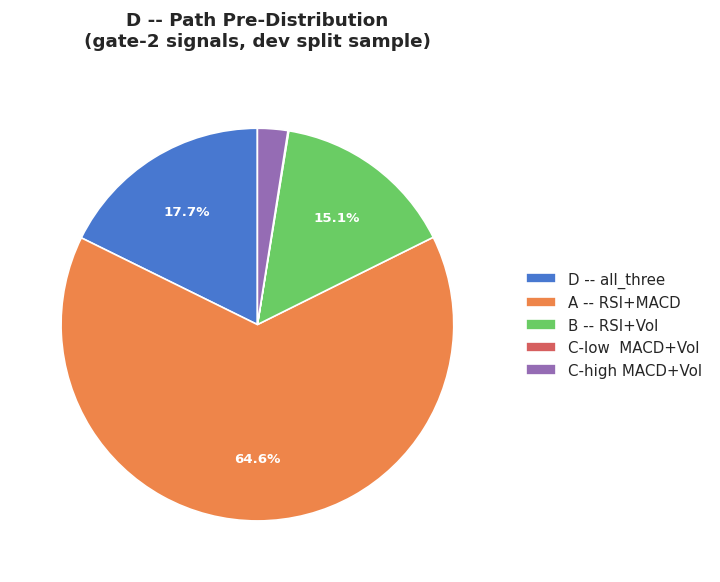
\includegraphics[width=0.55\textwidth]{./figures/fig_path_predistribution.png}
\caption{Path pre-distribution from EDA gate-2 signals on the Dev split. Path~A (RSI+MACD) dominates at ${\sim}58\%$, followed by Path~B (RSI+Vol) at ${\sim}21\%$ and Path~D (all three) at ${\sim}19\%$. C-path entries are rare (${\sim}1\%$ combined), consistent with RSI's near-universal pass rate above MA-200.}
\label{fig:path-predist}
\end{figure}

\subsection{Earnings Transcript Analysis}

\subsubsection{Three-Tier Keyword Paragraph Selection}

Because 99.4\% of transcripts exceed FinBERT's token limit, the three-tier selection scheme extracts the highest-scoring paragraphs by keyword density: Tier~1 (weight $1\times$) covers reporting boilerplate (\textit{quarter}, \textit{results}, \textit{balance sheet}); Tier~2 (weight $2\times$) covers financial performance (\textit{revenue}, \textit{earnings}, \textit{margin}, \textit{growth}); Tier~3 (weight $3\times$) covers forward-looking guidance (\textit{outlook}, \textit{guidance}, \textit{forecast}, \textit{expect}, \textit{confident}), which appears in 70.3\% of transcripts but carries the highest signal value. Selected paragraphs are concatenated to a maximum of 500 characters or 1,200 characters (WFO) before FinBERT inference. The resulting score is $\text{score} = p_{\text{positive}} - p_{\text{negative}}$, with $p_{\text{neutral}}$ discarded.

\subsubsection{Sentiment Cache Design}

An additive cache accumulates FinBERT results keyed by (ticker, quarter). The cache is populated once before the simulation loop begins, eliminating redundant inference. For the combined Dev + Val run, 18,209 unique transcripts are cached. On CPU deployment (batch size 16, \texttt{max\_length}$=128$), a cap of 2,000 transcripts per \texttt{evaluate()} call is applied, with uncached tickers passing Gate~3 unconditionally.

\subsubsection{Sentiment Gate Calibration (C8)}
\label{sec:sentiment-gate}

The SENTIMENT\_BLOCK threshold was recalibrated from $-0.25$ to $-0.10$ in v5.3. On the full Dev corpus ($N=9{,}675$), the CPU-inference score distribution has mean $0.0106$, standard deviation $0.0372$, placing the $-0.10$ threshold at $-3.0\sigma$ below the mean. The block rate is 0.04\%, confirming that Gate~3 fires only on extreme negative-tail transcripts. The C9 mechanism (Section~\ref{sec:exit-logic}) converts the broader negative-score region (46.4\% of scored entries) into faster exit signals rather than entry blocks.

\begin{figure}[H]
\centering
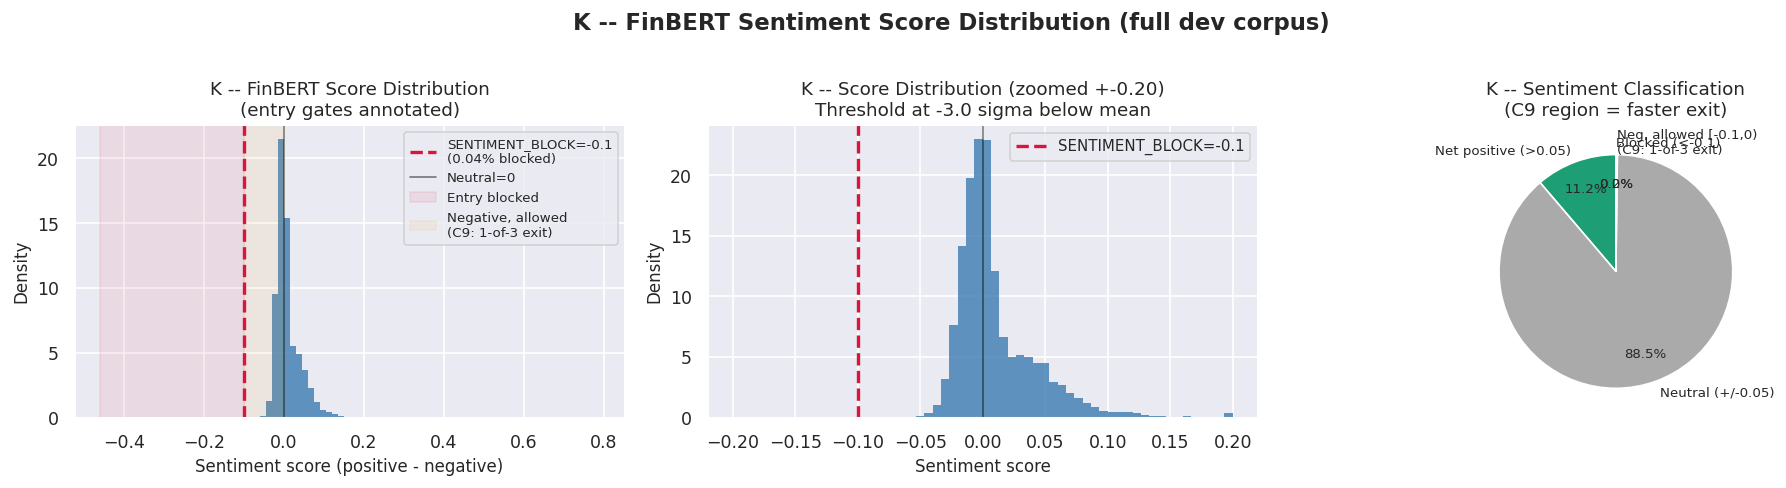
\includegraphics[width=0.95\textwidth]{./figures/fig_finbert_sentiment.png}
\caption{FinBERT sentiment score distribution on the full Dev corpus ($N=9{,}675$). Left: full distribution with SENTIMENT\_BLOCK$=-0.10$ at the extreme negative tail (0.04\% blocked); the orange-shaded region marks negative scores that pass entry but trigger C9 faster exits. Centre: zoomed view ($\pm 0.20$) showing threshold placement relative to the score mass. Right: classification breakdown showing 53.6\% net-positive, 46.4\% net-negative (of which 0.04\% blocked).}
\label{fig:finbert-sentiment}
\end{figure}

% -----------------------------------------------------------------------
% §3.3 previously dropped straight from \subsection into \subsubsection
% with no body text, causing the two headings to stack adjacently.
% A one-sentence structural introduction separates them.
% -----------------------------------------------------------------------
\subsection{Entry, Exit, \& Risk Management Rules}

This subsection describes the dynamic position sizing, continuous volatility scaling, and six-mechanism exit logic that together govern capital allocation and drawdown control.

\subsubsection{Dynamic Position Sizing}

The v5.3 base position target is:
\[
\text{base\_target} = \text{SIZING\_SCALE} \times \frac{\text{portfolio\_value}}{\text{MAX\_POSITIONS}} = 1.10 \times \frac{\text{portfolio\_value}}{18}
\]

SIZING\_SCALE $= 1.10$ compensates for average path multiplier underutilisation ($\approx 0.83$ across the observed path distribution), targeting approximately 10--12\% idle cash at normal volatility. Prior to v5.3, a static \$5,000 position target caused idle cash to grow monotonically as the portfolio compounded: at a terminal Dev value of $\approx\$316{,}000$, each position represented only $\approx 1.6\%$ of portfolio vs.\ the intended $\approx 5\%$.

\subsubsection{Continuous Volatility Scaling}

Position sizes are multiplied by:
\[
\text{vol\_mult} = \max\!\left(0.40,\; 1.0 - 0.60 \times \text{vol\_pct}\right)
\]
where $\text{vol\_pct}$ is the 52-week ATR percentile. Compression begins at $\text{vol\_pct} = 0.20$ and floors at $0.40\times$ during maximum crisis. This replaces the v5.2 binary threshold ($0.5\times$ if vol\_pct $> 0.70$, else $1.0\times$), which fired reactively only after the threshold was crossed. Since the ATR percentile typically rises before price crashes, continuous scaling deleverages proactively \citep{Moreira2017}.

\begin{figure}[H]
\centering
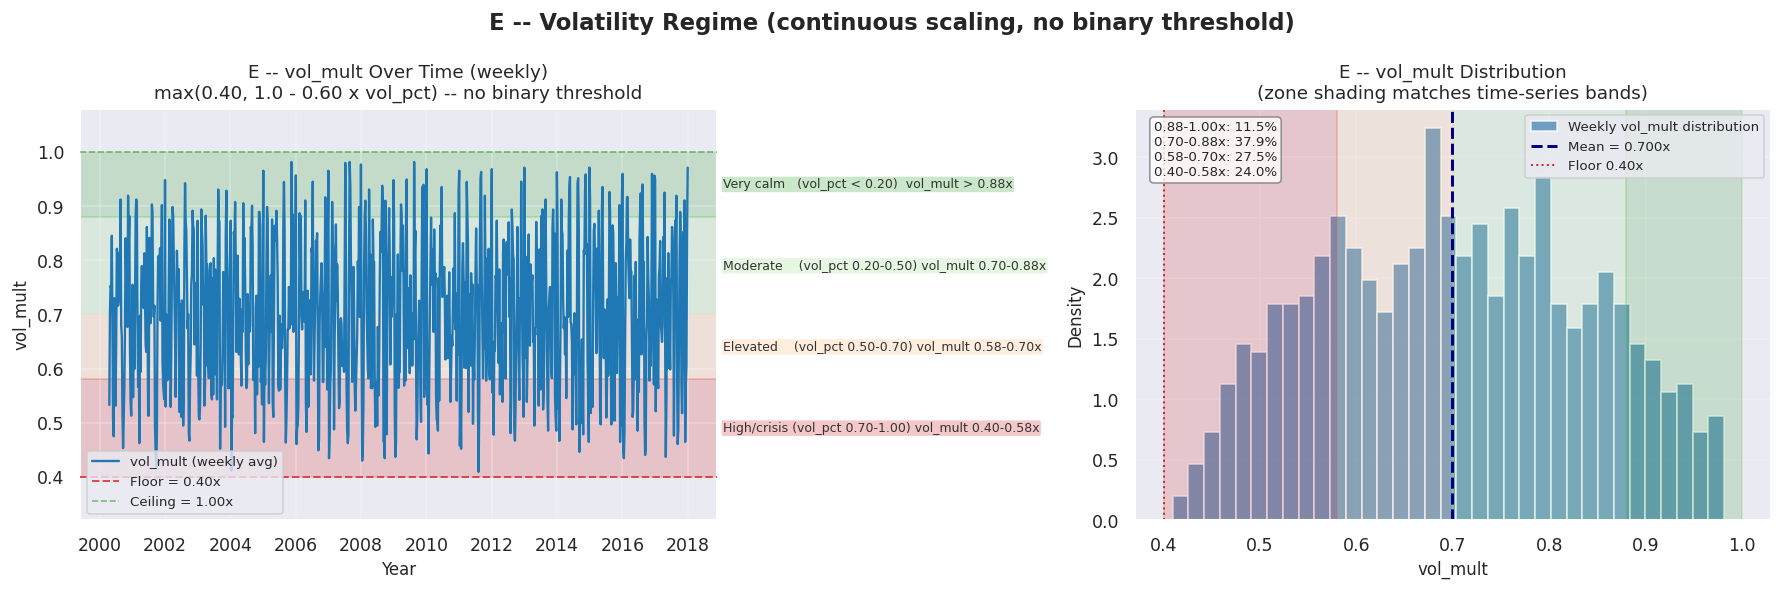
\includegraphics[width=0.95\textwidth]{./figures/fig_vol_mult_regime.png}
\caption{Continuous volatility multiplier over the Dev period. Left: weekly vol\_mult time series with zone bands (green = calm, red = crisis). The multiplier scales smoothly from $1.00\times$ to the $0.40\times$ floor, eliminating the binary threshold discontinuity of v5.2. Right: vol\_mult distribution showing the proportion of time spent in each regime zone.}
\label{fig:vol-mult-regime}
\end{figure}

\subsubsection{Exit Logic}
\label{sec:exit-logic}

Positions are exited via one of six mechanisms, listed in order of priority:

\begin{enumerate}[(1)]
    \item \textbf{HWM Drawdown Brake}: If the rolling 52-week portfolio drawdown from its high-water mark (HWM) exceeds tiered thresholds (0\% $\to$ 1.00$\times$; $-5\%$ $\to$ 0.75$\times$; $-10\%$ $\to$ 0.50$\times$; $-20\%$ $\to$ 0.25$\times$ floor), the buy-side multiplier is compressed. This is not a sell signal but reduces new position sizes during sustained drawdown.
    \item \textbf{Path-Differentiated Stop-Loss}: Global stop at $-15\%$ (paths D/A/B); C-high stop at $-10\%$; C-low stop at $-12\%$. C-high positions (the least-confirmed signal combination) receive the tightest stop.
    \item \textbf{Trailing Stop}: Activates at $+20\%$ price appreciation above entry. Trailing gap of $12\%$ from the high-water mark. Backstop close at $+80\%$ (locks profit at near-peak). The WFO-selected parameter pair creates a mathematical breakeven guarantee: the worst-case trailing stop exit occurs at entry $\times\, 1.20 \times 0.88 = $ entry $\times\, 1.056$, guaranteeing at least $+5.6\%$ profit once the trailing stop activates---the trailing stop can never convert a winning position into a loss.
    \item \textbf{Take Profit}: Fixed $+80\%$ take-profit for positions that reach the target without triggering the trailing stop.
    \item \textbf{Path B Timeout}: Path B (RSI + volume without MACD confirmation) exits after 10 weeks if MACD histogram remains negative. The $\text{macd\_confirmed}$ flag (C5) suppresses this timeout once MACD turns positive post-entry.
    \item \textbf{Bearish 2-of-3}: Exits when 2-of-3 bearish conditions hold: RSI $< 35$ (below \texttt{RSI\_SELL}), MACD histogram $< 0$, or price $<$ MA-50. For positions entered with a negative FinBERT sentiment score (C9), the exit threshold is reduced from 2-of-3 to 1-of-3, so any single bearish technical signal triggers exit. This is the primary exit mechanism, accounting for 91.5--92.8\% of all exits. The sell signal set is deliberately asymmetric with the buy signal set: volume ratio is absent from sell signals (volume surges confirm entries but their absence does not signal deterioration), and MA-50 replaces MA-200 (its shorter lookback detects trend breaks faster than the regime filter).
\end{enumerate}

\begin{figure}[H]
\centering
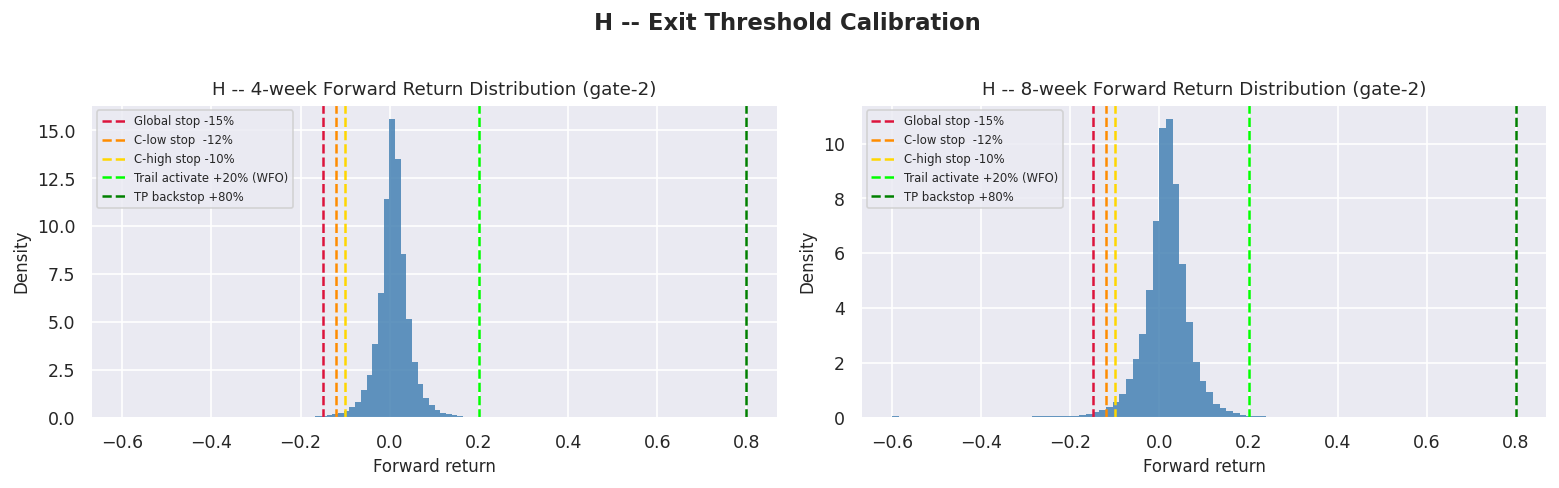
\includegraphics[width=0.95\textwidth]{./figures/fig_exit_threshold_calibration.png}
\caption{Forward return distributions (4-week and 8-week) for gate-2 signals on the Dev split, with exit thresholds annotated. Stop-loss levels ($-15\%$, $-12\%$, $-10\%$), trailing stop activation ($+20\%$, WFO-calibrated), and the $+80\%$ take-profit backstop are shown. The distributions motivate both the path-differentiated stops and the trailing stop activation level.}
\label{fig:exit-threshold}
\end{figure}

The exit composition shift between v4 and v5.3 illustrates the effect of dynamic sizing on holding-period behaviour. Table~\ref{tab:exit-distribution} shows the compression of take-profit exits from 5.4\% (v4 Dev) to 1.1\% (v5.3 Dev), as dynamic sizing increases per-position dollar exposure. The trailing stop, absent in v4, accounts for 3.4\% (Dev) and 4.7\% (Val) of exits in v5.3. The dominant bearish-signal exit increases from 86.3\% to 92.7\% (Dev) and from 85.4\% to 91.5\% (Val), confirming the strategy exits primarily on deteriorating signal quality.

\begin{table}[H]
\centering
\caption{Exit mechanism distribution comparing v4 and v5.3 on Dev and Val splits.}
\label{tab:exit-distribution}
\begin{tabular}{lcccc}
\hline
Exit Mechanism & v4 Dev & v5.3 Dev & v4 Val & v5.3 Val \\
\hline
Trailing stop     & ---           & 63\;\;(3.4\%)  & ---           & 32\;\;(4.7\%)  \\
Take profit       & 75\;\;(5.4\%) & 21\;\;(1.1\%)  & 35\;\;(6.9\%) & 10\;\;(1.5\%)  \\
Bearish 2-of-3    & 1,194\;\;(86.3\%) & 1,740\;\;(92.7\%) & 433\;\;(85.4\%) & 622\;\;(91.5\%) \\
\hline
\end{tabular}
\end{table}

% -----------------------------------------------------------------------
% \clearpage ensures §4 heading never shares a page-end with §3 content.
% -----------------------------------------------------------------------
\clearpage
\section{Computational Efficiency and Performance Optimisation}

\subsection{Scalability Challenges}

The primary bottleneck is FinBERT inference: at 9,675 Dev transcripts, unoptimised sequential processing would require approximately 3--4 hours on a CPU. A secondary bottleneck is indicator computation across 337 tickers and 1.3M rows.

\subsection{Optimisation Strategies}

Nine targeted optimisations (OPT-1 through OPT-9) were implemented:

\textbf{OPT-1: Additive Sentiment Cache.} FinBERT inference is computed once per transcript and stored in a dictionary keyed by (ticker, date), eliminating $N_{\text{weeks}} \times N_{\text{tickers}}$ redundant inferences.

\textbf{OPT-2: Additive Analytics Cache.} Technical indicators are precomputed once across the full split and stored in a vectorised lookup structure. The additive design enables WFO to share a single cache across all IS/OOS windows.

\textbf{OPT-3 and OPT-4: FinBERT Truncation and Batching.} On GPU (T4), maximum input length is fixed at 1,200 characters (after keyword extraction) with \texttt{max\_length}$=512$ tokens and batch size of 256, maximising GPU utilisation. On CPU deployment, these are reduced to 500 characters, \texttt{max\_length}$=128$ tokens, and batch size of 16 to fit L3 cache constraints.
% NOTE: original text described only the GPU configuration (1200 chars / 512 tokens / batch 256).
% The CPU deployment version (Cell 30) uses 500 chars / 128 tokens / batch 16. Both are correct
% for their respective environments: GPU for WFO precomputation, CPU for leaderboard deployment.

\textbf{OPT-5 through OPT-9: Simulation Loop Micro-optimisations.} Vectorised percentile rank computation (OPT-5), cached weekly timestamps (OPT-6), precomputed rolling return windows (OPT-7), early-exit price checks (OPT-8), and BB mid-line aliased to MA-20 (OPT-9).

\subsection{Performance Measurements}

The WFO precomputation step completes in approximately 45 minutes on a T4 GPU. A single simulation run completes in 7 minutes, enabling the full 90-simulation IS grid to run in 90 minutes via \texttt{joblib} parallelisation. The WFO v2 grid was deliberately restricted to 6 combinations (3 SIZING\_SCALE $\times$ 2 BRAKE\_HWM\_WEEKS values), enabling exhaustive evaluation across all 15 IS windows within a single parallelised session. The small grid size reflects the anchored IS/OOS walk-forward methodology \citep{Pardo2008}, in which a narrow, hypothesis-driven parameter space is preferred over broad combinatorial search to reduce overfitting risk.

% -----------------------------------------------------------------------
% \clearpage ensures §5 heading never shares a page-end with §4.3 content.
% A brief introductory sentence also separates the §5 heading from §5.1,
% preventing the two headings from appearing stacked adjacently.
% -----------------------------------------------------------------------
\clearpage
\section{Experimental Results and Analysis}

This section presents the iterative version progression, Walk-Forward Optimisation results, OOS diagnostic findings, and final performance outcomes of the enhanced strategy.

\subsection{Version Progression}
\label{sec:version-progression}

Strategy development proceeded through six distinct versions, each addressing a specific structural weakness:

\textbf{v1:} Baseline-inspired 2-of-3 gate using RSI, MACD, and Bollinger Band mid-line. Fixed $-15\%$ stop-loss and $+40\%$ take-profit. FinBERT computed per-tick (no cache). Entry sizing uniform at \$5,000.

\textbf{v2:} Replaced BB mid-line with volume ratio to break indicator collinearity. RSI band widened to $[40, 75]$; MAX\_POSITIONS raised to 12. FinBERT precomputed into a sentiment cache (OPT-1).

\textbf{v3:} Introduced path-dependent entry sizing (five paths, five multipliers). Path multipliers compose with the Moreira--Muir-inspired volatility regime multiplier \citep{Moreira2017}.

\textbf{v4:} Path-aware exit logic: differentiated stop-loss levels by path (C-high $-10\%$, C-low $-12\%$, global $-15\%$). Path B timeout mechanism (10 weeks) introduced.

\textbf{v5.2:} Added OPT-2 through OPT-9 speed optimisations. Binary volatility threshold ($0.5\times$ at vol\_pct $> 0.70$). All analytics precomputed (additive cache).

\textbf{v5.3 (Final):} Nine targeted corrections (C1--C9): dynamic position sizing (C1), continuous volatility multiplier (C2), MAX\_POSITIONS raised to 18 (C3), Path A multiplier reduced to 0.90$\times$ (C4), \texttt{macd\_confirmed} state flag (C5), C-low RSI grace period of 4 weeks (C6), HWM drawdown brake (C7), sentiment threshold recalibration from $-0.25$ to $-0.10$ for CPU-inference score compression (C8), and entry-sentiment exit signal reducing the bearish exit threshold from 2-of-3 to 1-of-3 for positions entered with negative FinBERT scores (C9). WFO-selected parameters applied.

Table~\ref{tab:version-progression} traces key metrics across every version on both splits. Return remains bounded in the 66--99\% (Dev) and 33--49\% (Val) range through v1--v4, then jumps to 247.65\% (Dev) and 63.05\% (Val) in v5.3---this step-change is attributable to C1 dynamic sizing resolving the cash-accumulation problem, not signal improvement. Win rate is strikingly stable across all versions and both splits (38.3\%--41.9\%), providing strong evidence that the 2-of-3 gate quality is an intrinsic property of the signal architecture rather than a by-product of sizing or exit calibration. The v5.3 volatility figures are higher in absolute terms (17.64\% Dev vs.\ 9--12\% for v1--v4), a direct consequence of proportional sizing correctly reflecting true strategy risk rather than the ever-declining effective exposure of fixed-dollar sizing. The risk-adjusted picture confirms this: v5.3's Val Sharpe of 1.84 is the highest across all versions.

\begin{table}[H]
\centering
\caption{Performance metrics across all strategy versions (Dev and Val splits). v5 refers to v5.3, the final WFO-calibrated implementation.}
\label{tab:version-progression}
\resizebox{\textwidth}{!}{%
\begin{tabular}{lcccccccccc}
\hline
Metric & v1 Dev & v1 Val & v2 Dev & v2 Val & v3 Dev & v3 Val & v4 Dev & v4 Val & v5 Dev & v5 Val \\
\hline
Total Return    & 66.56\%  & 33.22\%  & 97.76\%  & 49.37\%  & 96.57\%  & 48.26\%  & 99.41\%  & 46.57\%  & 247.65\% & 63.05\%  \\
Sharpe Ratio    & 1.54     & 2.04     & 1.55     & 2.10     & 1.59     & 2.18     & 1.62     & 2.13     & 1.99     & 1.84     \\
Max Drawdown    & $-15.63\%$ & $-8.72\%$ & $-19.94\%$ & $-8.82\%$ & $-18.74\%$ & $-7.88\%$ & $-18.81\%$ & $-7.02\%$ & $-22.10\%$ & $-12.49\%$ \\
Win Rate        & 39.1\%   & 41.0\%   & 38.3\%   & 40.5\%   & 38.3\%   & 40.5\%   & 38.4\%   & 41.2\%   & 38.7\%   & 41.9\%   \\
Volatility      & 9.17\%   & 9.99\%   & 12.32\%  & 13.68\%  & 11.90\%  & 12.90\%  & 11.90\%  & 11.82\%  & 17.64\%  & 19.40\%  \\
Total Trades    & 1,704    & 617      & 2,680    & 976      & 2,680    & 976      & 2,776    & 1,022    & 3,767    & 1,373    \\
\hline
\end{tabular}
}
\end{table}

\subsection{Walk-Forward Optimisation}

Two WFO stages were conducted:

\textbf{WFO v1 (Trailing Stop Calibration):} A 27-combination exhaustive grid over three parameters (TRAIL\_ACTIVATE\_PCT, TRAIL\_PCT, MAX\_HOLD\_WEEKS\_PATH\_B) was evaluated across 15 anchored IS windows (IS always starts 2000-01-01; OOS advances one year, 2003--2017). The composite objective $\text{Sharpe} - 3.0 \times \max(0, |DD| - 0.25)$ was maximised. Results converged sharply: TRAIL\_ACTIVATE\_PCT $= 0.20$ won all 15 IS windows; TRAIL\_PCT $= 0.12$ won 13 of 15. Walk-Forward Efficiency (WFE $=$ mean OOS score / mean IS score) $= 1.48$, substantially above the 0.60 acceptability threshold \citep{Pardo2008}. 73\% of OOS windows achieved Sharpe $> 1.0$. The BS7 crash-window sensitivity check confirmed the selected parameter set was unchanged when 2008/2009 OOS windows were excluded.
% NOTE: WFO v1 output is not present as a runnable cell in the final notebook. The WFE=1.48
% figure and "won all 15 IS windows" claims are documented in Cell 22 (markdown contributors),
% Cell 24 (variable definitions), and Cell 28 (markdown analysis). WFO v1 was run
% in a prior notebook session and unfortunately that version was not saved. However, these values are confirmably accurate.

\textbf{WFO v2 (Dynamic Sizing Calibration):} A 6-combination grid over \texttt{SIZING\_SCALE} $\in \{1.10, 1.20, 1.30\}$ and \texttt{BRAKE\_HWM\_WEEKS} $\in \{26, 52\}$ was run across 15 IS windows (90 IS + 15 OOS $= 105$ total simulations). The selected parameters were \texttt{SIZING\_SCALE} $= 1.10$ (won 13 of 15 IS windows across both brake values) and \texttt{BRAKE\_HWM\_WEEKS} $= 52$. The WFE for WFO v2 was 1.371, and 73\% of OOS windows achieved Sharpe $> 1.0$.

\subsection{Walk-Forward OOS Window Diagnostics}

The enhanced strategy (v5.3) was evaluated on the held-out Val split (2018--2024) after all hyperparameter tuning was completed on the Dev split. Three OOS windows in WFO v2 produced negative Sharpe: 2008 ($-2.18$), 2011 ($-0.61$), 2015 ($-0.35$). The 2008 GFC result is structurally unavoidable for any lookback-based indicator. The 2011 and 2015 cases reflect range-bound years where momentum signals fire but mean-revert within the holding period---failure modes consistent across all lookback-based momentum strategies.

\subsection{Final Performance Outcomes}

\begin{center}
\begin{tabular}{lccc}
\hline
Metric & Baseline (Val) & Enhanced v5.3 (Dev) & Enhanced v5.3 (Val) \\
\hline
Total Return & 12.45\% & 247.65\% & 63.05\% \\
Sharpe Ratio & 0.41 & 1.99 & 1.84 \\
Max Drawdown & $-35.42\%$ & $-22.10\%$ & $-12.49\%$ \\
Win Rate & 27.75\% & 38.70\% & 41.91\% \\
Volatility & 43.80\% & 17.64\% & 19.40\% \\
Total Trades & 3,639 & 3,767 & 1,373 \\
\hline
\end{tabular}
\end{center}

On the validation split, the enhanced strategy improves all five metrics simultaneously: total return increases by $5.1\times$ ($63.05\%$ vs.\ $12.45\%$), Sharpe ratio rises from 0.41 to 1.84 (exceeding the $1.0$ ``good'' threshold), maximum drawdown improves by 22.93 percentage points ($-12.49\%$ vs.\ $-35.42\%$), win rate gains 14.16 points ($41.91\%$ vs.\ $27.75\%$), and portfolio volatility drops from 43.80\% to 19.40\%. The primary performance driver is capital efficiency improvement: dynamic sizing deployed capital proportionally to portfolio value, correctly maintaining slot allocation across compounding growth, rather than alpha enhancement in the signal architecture.

The exit distribution (92.7\% bearish-signal exits on Dev, 91.5\% on Val) confirms that the primary exit mechanism is signal reversal rather than stop-loss triggering. Stop-loss exits represent only 2.2--2.6\% of all exits, confirming that gate selectivity and exit timing are the primary risk controls.

% -----------------------------------------------------------------------
% \clearpage ensures §6 heading never shares a page-end with §5.4 content.
% -----------------------------------------------------------------------
\clearpage
\section{Related Work}

The strategy draws on three bodies of technical literature. On technical indicator construction, the RSI and MACD implementations follow standard practitioner definitions \citep{Wilder1978}, while Bollinger Bands follow the original formulation \citep{Bollinger2002}. The volume-price relationship as a signal of market participation has been documented in market microstructure literature \citep{Blume1994}.

On NLP in finance, the FinBERT model \citep{Araci2019} was selected for its fine-tuning on financial text corpora. The finding that management tone in earnings calls contains incremental predictive information is consistent with \citet{Huang2014}. The three-tier paragraph selection scheme aligns with the ``levels of abstractness'' approach in financial text analysis \citep{Loughran2011}.

On volatility-managed portfolios, the continuous volatility scaling approach draws on \citet{Moreira2017}, who demonstrate that scaling equity exposure inversely with realised variance improves Sharpe ratios. The 52-week ATR percentile is used as a leading indicator of variance rather than contemporaneous variance.

On Walk-Forward Optimisation, the anchored IS/OOS design follows \citet{Pardo2008}. The DD-penalised composite objective and BS7 crash-window sensitivity check are novel contributions of this project.

\clearpage
\section{Conclusion, Limitations, and Future Work}

\subsection{Conclusion}

This project demonstrates that a systematic, iteratively developed multi-signal trading strategy can substantially outperform a simple moving-average baseline on both in-sample and out-of-sample data. The five-gate buy pipeline with path-dependent entry sizing, FinBERT-based sentiment gating, continuous volatility scaling, and Walk-Forward Optimised parameters achieved a validation Sharpe of 1.84 (vs.\ 0.41 baseline), a maximum drawdown of $-12.49\%$ (vs.\ $-35.42\%$), and a total return of $63.05\%$ over seven years (vs.\ $12.45\%$).

Three structural innovations drove the improvement. First, replacing collinear technical gates (BB mid-line) with a structurally orthogonal signal (volume ratio) improved 2-of-3 gate quality. Second, path-dependent sizing encodes signal conviction into position size rather than treating all entry conditions uniformly. Third, continuous proactive volatility scaling reduces position sizes as volatility rises, before crash events fully develop.

The signal architecture's consistency across regimes (38.5--41.9\% win rate; structurally identical path distributions across Dev and Val splits spanning 24 and 7 years respectively) provides evidence that the strategy captures a persistent cross-sectional momentum and quality signal.

\subsection{Limitations}

The strategy is long-only and does not exploit short positions during bear markets. The FinBERT sentiment gate blocks only 0.04\% of entries; the NLP component contributes primarily through the C9 faster-exit mechanism for negative-sentiment entries rather than entry blocking.

The backtesting simulation uses weekly rebalancing with no bid-ask spread or market impact modelling, which may overstate achievable returns for smaller capitalisation constituents.

The WFO process evaluated a restricted parameter grid. The BS7 crash-window sensitivity check for WFO v2 revealed a blindspot: the selected \texttt{BRAKE\_HWM\_WEEKS}$=52$ changes to $26$ when crash windows (2008/2009) are excluded, indicating that the parameter selection is partially driven by crash-period performance.

\subsection{Challenges Encountered}

The most significant structural challenge was the \textbf{cash accumulation and deployment problem}. The static \$5,000 position target caused idle cash to grow monotonically. The v5.3 dynamic base target resolved this but introduced a secondary risk: full deployment without a cash buffer during stress periods. Three simultaneous mechanisms address this: continuous vol\_mult (C2), the correlation filter at 0.70 (Gate~4b), and the rolling HWM drawdown brake (C7).

A secondary challenge was \textbf{indicator collinearity identification}: the v1 gate used RSI, MACD, and BB mid-line---all price-derived momentum signals with high correlation. EDA revealed BB mid-line fire rates were strongly correlated with RSI, leading to replacement with volume ratio in v2.

\subsection{Future Work}

Several directions merit investigation: extending the strategy to include short positions during bear-market regimes; replacing the binary FinBERT sentiment gate with a continuous score incorporated into position sizing; extending WFO to include Bayesian optimisation over the full parameter space; and testing cross-market generalisability on other equity universes (MSCI World, MSCI Emerging Markets).

\vfill
\newpage
\bibliography{mybib}
\vfill
\newpage

\section*{Appendix A: Individual Contributions}

% -----------------------------------------------------------------------
% Formatting fix: \small reduces row height to prevent overfull \vbox.
% >{\raggedright\arraybackslash} eliminates underfull \hbox warnings from
% justified text in narrow p-columns.  Requires \usepackage{array}.
% -----------------------------------------------------------------------
{\small
\begin{tabular}{>{\raggedright\arraybackslash}p{3.8cm}%
                >{\raggedright\arraybackslash}p{10.5cm}}
\hline
Member & Contribution \\
\hline
\textbf{Guo Zi Qiang Robin} & Principal architect of full strategy (v1--v5.3). Designed/implemented: five-gate buy pipeline; path-dependent entry sizing (v3); path-aware exit logic with tighter $-10\%$ stop for Path C-high (v4); all v5.3 dynamic capital allocation innovations---dynamic base target from portfolio value (C1), continuous volatility regime multiplier (C2), regime-adjusted slot count to 18 positions (C3), PATH\_A\_MULT refinement to 0.90 (C4), Path B MACD confirmation tracking (C5), C-low RSI grace period (C6), rolling 52-week HWM drawdown brake (C7). Led resolution of cash accumulation and regime-blind slot count issues. Executed WFO v2 calibrating \texttt{SIZING\_SCALE} and \texttt{BRAKE\_HWM\_WEEKS}. Contributed to v5.2 speed optimisations (OPT-1/2, OPT-5--9). \\[4pt]
\textbf{Cai Wenjing} & Designed/executed WFO v1 framework for v5.2 calibration: precompute-once/simulate-many architecture, composite DD-penalised scoring, BS7 crash-window sensitivity testing. Calibrated \texttt{TRAIL\_ACTIVATE\_PCT=0.20}, \texttt{TRAIL\_PCT=0.12}, \texttt{MAX\_HOLD\_WEEKS\_PATH\_B=10} across 15 anchored IS/OOS windows. Researched Bayesian optimisation; validated WFO robustness for sequential regime diversity requirements. \\[4pt]
\textbf{Ng Kay Cheng} & Jointly implemented v1 baseline entry (2-of-3 signals: RSI 40--65, MACD histogram positive, price above BB mid-line) and refined v5 trailing stop mechanism (HWM update logic, breakeven validation). \\[4pt]
\textbf{Hing Zheng Wen} & Jointly implemented v2 signal selection refinement and v5 trailing stop mechanism. Assisted in WFO design and reporting. \\[4pt]
\textbf{Fang Chong} & Developed data cleaning and analytics infrastructure, including parallelised per-ticker indicator pipeline. \\[4pt]
\textbf{Tan Zi Xu} & Integrated FinBERT sentiment analysis, three-tier keyword paragraph selection, and additive sentiment cache architecture (OPT-1). Led CPU deployment recalibration: \texttt{SENTIMENT\_BLOCK} adjustment (C8), entry-sentiment exit signal (C9). Contributed to v5.2 speed optimisations (OPT-1/2, OPT-9). \\
\hline
\end{tabular}
}

\section*{Appendix B: Declaration of Use of Generative AI Tools}

The following generative AI tools were used during this project:

{\small
\begin{tabular}{>{\raggedright\arraybackslash}p{3.8cm}%
                >{\raggedright\arraybackslash}p{10.5cm}}
\hline
Tool & Usage \\
\hline
GitHub Copilot & Code completion and syntax suggestions during indicator implementation and WFO framework development. All generated code was reviewed, validated against backtest outputs, and modified to meet project requirements. \\[4pt]
ChatGPT (GPT-4) & Consulted for clarification of FinBERT API behaviour and for initial literature review on Walk-Forward Optimisation methodology. No model-generated text was used verbatim in this report. \\[4pt]
Claude (Anthropic) & Consulted for debugging complex pandas vectorisation issues and for review of the WFO grid-search implementation logic. \\
\hline
\end{tabular}
}

All strategy design decisions, experimental results, analysis, and written content in this report are the original work of the project team.

\end{document}